\documentclass[10pt, a4paper]{article}
\usepackage[utf8x]{inputenc}            % Acentos, ñ, etc.
\usepackage{graphicx}                   % Gráficos
\usepackage[spanish]{babel}             % Macros en español
\usepackage{caratula}                   % Carátula
\usepackage{float}
\begin{document}

%Caratula
\titulo{Trabajo Práctico 1}
\subtitulo{Detección de Spam}
\fecha{\today}
\materia{Aprendizaje Automático}
\integrante{Fernández, Gonzalo}{836/10}{gpfernandezflorio@gmail.com}
\integrante{Damian, Aleman}{377/10}{damianealeman@gmail.com}
\integrante{Matías, Pizzagalli}{257/10}{matipizza@gmail.com}



%Titulo e indice
\maketitle
\tableofcontents
\newpage

\section*{Introducción}

%\includegraphics{algo.png}
\section{Metodología}
Cargamos los mails de los archivos json
Extrajimos los atributos de la base de mails y los guardamos como matrices
Separamos los datos de entrenamiento de los de test utilizando la funciøn train\_test\_split y almacenamos cada conjunto en archivos npy.

\section{Extracción de atributos}
%Describir en castellano los atributos extraidos de los mails, en forma concisa.
Para saber que palabras identifican mejor a los mails de spam, implementamos un script que cuenta la cantidad de ocurrencias por palabra, relativa entre los mails de spam contra los de ham.
Es decir, para cada palabra en los archivos json este script devuelve la cantidad de apariciones de dicha palabra en el archivo de spam menos la cantidad de apariciones de la misma palabra en el archivo ham.
Este script está implementado en el archivo \texttt{wordCounter.py}. En el archivo \texttt{words-100.txt} se pueden ver las 100 palabras con mayor cantidad de ocurrencias relativa.

En principio usamos como atributos la cantidad de apariciones de estas palabras en cada mail. Por otro lado agregamos los atributos

\begin{itemize}
\item Cantidad de palabras en mayusculas.
\item Cantidad de palabras compuestas por numeros.
\item Cantidad de palabras escritas con la primera letra en mayuscula.
\item Cantidad de letras promedio por palabra.
\item Cantidad de letras maxima por palabra.
\end{itemize}

Se pudo observar que a médida que ibamos agregando atributos, el modelo predictivo obtenía un valor más alto de accuracy y rápidamente se pudo llegar al \%97 de accuracy.

\section{Modelos}
%Listar los algoritmos de aprendizaje elegidos para experimentar. Describir cualquier decisión que hayan tomado (p.ej., elección de hiperparámetros).
Utilizamos los siguientes algoritmos de aprendizaje y seteamos los hiperparámetros a partir de un \texttt{gridSearch}:

\begin{description}
\item [Decision Tree] max\_depth: 14 16 o None, min\_samples_split: 3, criterion: entropy
\item [Random Forest] max_depth: None, min\_smaples\_split: 4,5, criterion: entropy, max\_features: 95 , n_estimators: 80 
\item [Naive Bayes]
\item [Vecinos Más Cercanos(KNN)]  n_neighbors: 4, weights: distance
\item [Support Vector Machines (SVM)]
\end{description}


\section{Reducción de dimensionalidad}
Sobre técnicas de reducción de dimensionalidad usamos:

\begin{description}
\item [PCA]
\item [ICA]
\item [iPCA]
\item [REFCV] Con esta ténica vimos los atributos que ofrecen mayor poder predictivo
\end{description}

% Describir brevemente las técnicas empleadas.
\section{Resultados}
 %Describir los resultados conseguidos por los distintos modelos y conjuntos de atributos considerados. Preferentemente, resumir los resultados en tablas/figuras. Mencionar los tiempos de ejecución aproximados de cada técnica.

Vimos como varía la médida de F1 a médida que incrementamos la cantidad de componentes.
\begin{figure}[H]
\centering
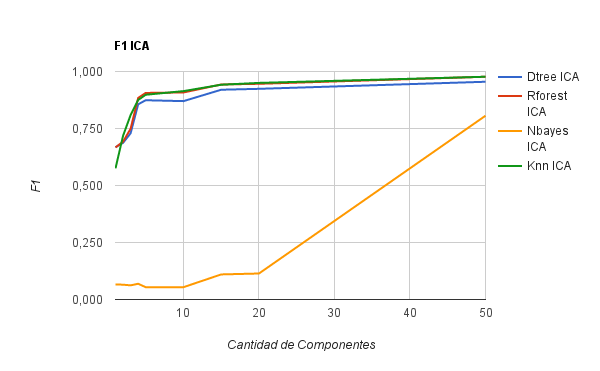
\includegraphics[width=\textwidth]{../imgs/F1ICA.png}
% \caption{}
% \label{fig:ej1}
\end{figure}

\begin{figure}[H]
\centering
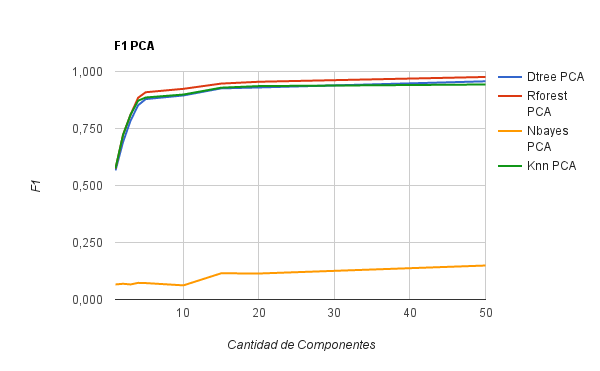
\includegraphics[width=\textwidth]{../imgs/F1PCA.png}
% \caption{}
% \label{fig:ej1}
\end{figure}

Comparamos los modelos según varias médidas de performance sobre los datos de test separados previamente (teniendo al mismo set de datos de test siempre para realizar las mediciones de forma adecuada):
\begin{figure}[H]
\centering
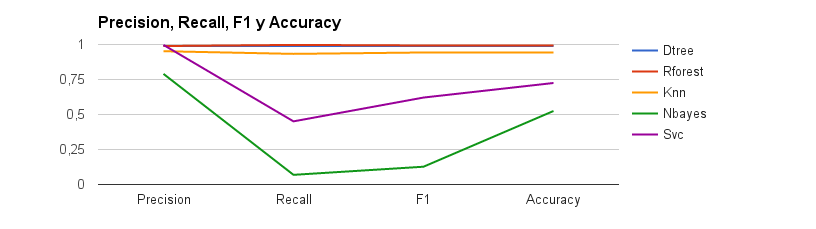
\includegraphics[width=\textwidth]{../imgs/metodos1.png}
% \caption{}
% \label{fig:ej1}
\end{figure}

\begin{figure}[H]
\centering
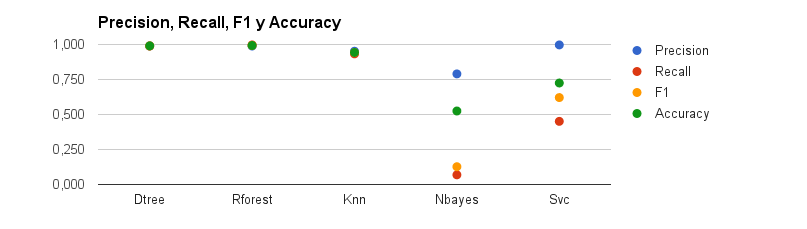
\includegraphics[width=\textwidth]{../imgs/metodos2.png}
% \caption{}
% \label{fig:ej1}
\end{figure}
A continuación mostramos un gráfico que muestra la médida de F1 en función de la cantidad de iteraciones del modelo de Support Vector Machine:
\begin{figure}[H]
\centering
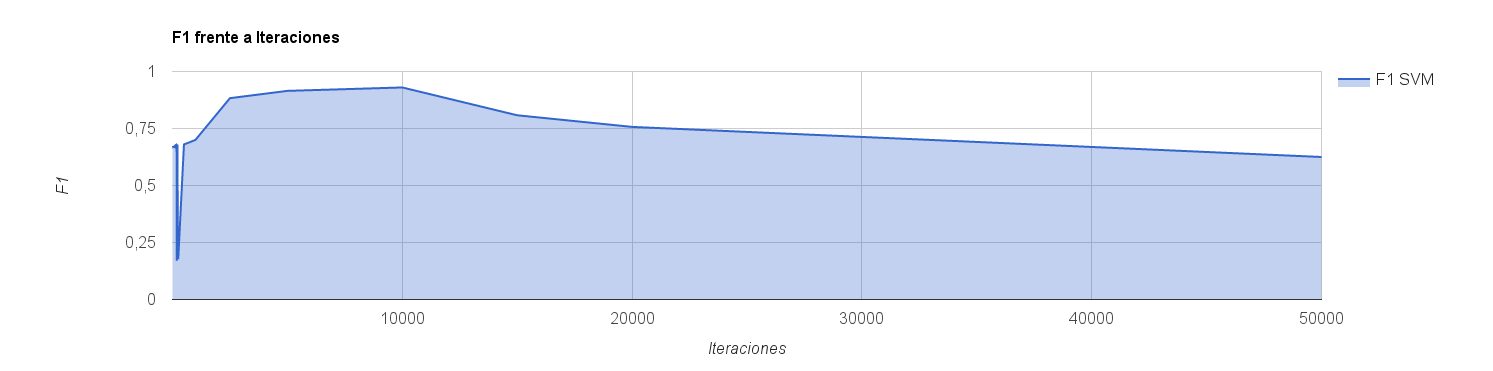
\includegraphics[width=\textwidth]{../imgs/SVCFULL.png}
% \caption{}
% \label{fig:ej1}
\end{figure}

\begin{figure}[H]
\centering
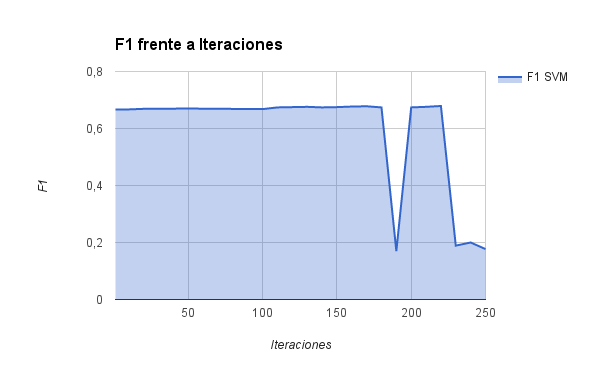
\includegraphics[width=\textwidth]{../imgs/SVCSTART.png}
% \caption{}
% \label{fig:ej1}
\end{figure}

%

\section{Discusión}
 %Analizar los resultados, buscando responder cuestiones como, por ejemplo: ¿cuáles son los atributos encontrados con mayor poder predictivo?, ¿cuán sensibles fueron los algoritmos a las técnicas de reducción de dimensionalidad consideradas?, ¿resultó clara la elección del algoritmo para la competencia, o hubo que poner en la balanza distintos factores?

 A continuación podemos ver los atributos con mayor poder predictivo seleccionados con el metodo de RFCV haciendo cross validation con k = 5 y step = 1. RFECV lo que hace es ir reduciendo la cantidad de atributos teniendo en cuenta un peso asociado que se obtiene a partir del estimador usado:

\begin{description}
\item [\texttt{count\_ESMTP}]
\item [\texttt{count\_upper}]
\item [\texttt{count\_guionba}]
\item [\texttt{count\_dol}]
\item [\texttt{count\_arr}]
\item [\texttt{count\_and}]
\item [\texttt{count\_equal}]
\item [\texttt{count\_dotc}]
\item [\texttt{count\_com}]
\item [\texttt{count\_menor}]
\item [\texttt{count\_menos}]
\item [\texttt{count\_html}]
\item [\texttt{count\_0600}]
\item [\texttt{count\_2002}]
\item [\texttt{count\_your}]
\item [\texttt{count\_0800}]
\item [\texttt{count\_align}]
\item [\texttt{count\_0500}]
\item [\texttt{count\_smtp}]
\item [\texttt{count\_cec}]
\end{description}


En el siguiente gráfico mostramos que con 20 atributos se puede llegar al score optimo de cross validation.
\begin{figure}[H]
\centering
% \includegraphics[width=145mm]{imgs/e3.jpg}
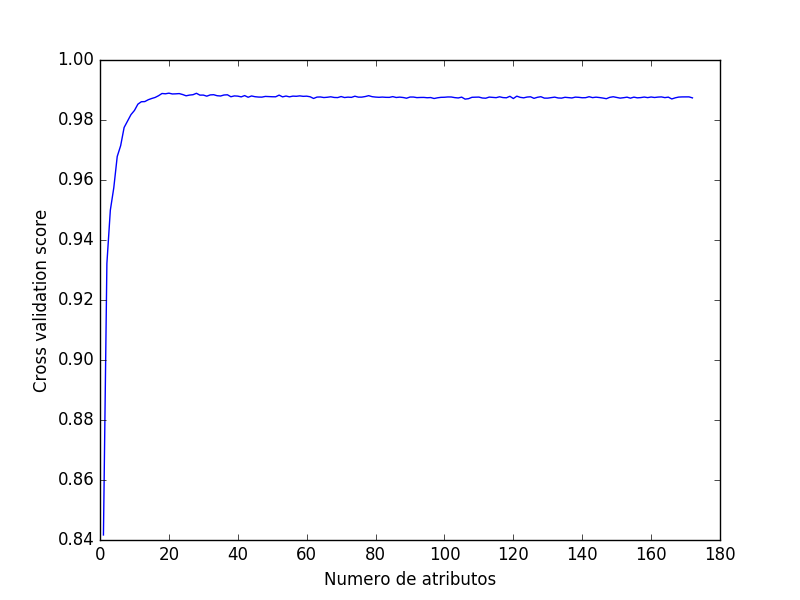
\includegraphics[width=\textwidth]{../imgs/atr.png}
% \caption{}
% \label{fig:ej1}
\end{figure}


% Podemos ver un græfico con medidas de cuan bueno es un modelo con pocas componentes y como mejora a lo largo del incremento de componentes

Notamos en el gráfico que compara F1 en función de la cantidad de componentes que con pocas componentes (5 o 6) ya se puede obtener un valor igual a 0,90 y después las demás componentes (de la nueva base transformada) no mejoran demasiado la médida de performance en cuestión.

Se puede observar que el mejor modelo es el de Random Forest, teniendo todas las médidas de performance en \%99. Igualmente el modelo basado en arboles de decisión es muy cercano en cuanto a performance, no así los modelos implementados de Naive Bayes y de Support Vector Machines. Por último el modelo de Vecinos más cercanos tiene un \%94 de accuracy. Dado que sabemos que Random Forest tuvo mejores médidas (incluso teniendo en cuenta el desvío estandard) lo elegimos como el modelo para ser usado en la competencia.

Por ultimo es importante destacar que el modelo SVM mejora hasta una cierta cantidad de iteraciones (aproximadamente 10000) y luego la performance empieza a disminuir.

\end{document}
